\chapter{Vulnerabilità implementazioni DDS}

In questo capitolo verranno mostrate dei casi studio
di tre tipologie di 
attacco che vengono effettuati tramite delle 
implementazioni del DDS dei vari vendors.

L'obiettivo di questi casi studio é di trovare delle 
vulnerabilitá in Robot Operating System (ROS) 2 che 
utilizza come middleware il DDS e come wire-protocol 
l'RTPS (Real-Time Publish-Subscribe Protocol).
Infatti saranno proprio i pacchetti RTPS a contenere 
l'exploit vero e proprio. Prima di mandare questi 
pacchetti é stato necessario creare una libreria Python 
così da poter automatizzare il loro processo di creazione.
Questo strumento, successivamente é stato anche unito al 
progetto Scapy di Python.

\begin{figure}[H]
    \centering
    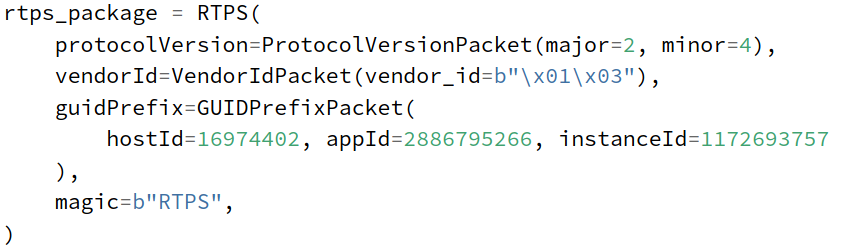
\includegraphics[width=15.2cm, keepaspectratio]{img/rptspacketheaderscapy.png}
    \caption{Un pacchetto RTPS.}
    \label{rptspacketheaderscapy}
\end{figure}

\section{Ricognizione DDS}
Le implementazioni DDS, per rispettare lo standard 
OMG, devono rispettare delle regole di interoperabilità 
per far si che i vari applicativi DDS siano compatibili 
tra di loro. Questo a portato alla creazione di un sistema
molto verbose per effettuare discovery 
di altri partecipanti all'interno di un network DDS.


La natura molto verbose del processo di discovery 
fa si che inviando un singolo pacchetto RTPS vuoto 
a un'entità di una rete DDS all'interno di un dominio 
quest'ultima risponderá 
con un messaggio discovery. La risposta ci permette di 
confermare se quel determinato partecipante é attivo.

\begin{figure}[H]
    \centering
    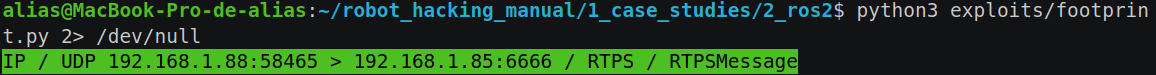
\includegraphics[width=15.2cm, keepaspectratio]{img/rispostarecoinnassance.png}
    \caption{Esempio di risposta discovery di un'entità DDS.}
    \label{rispostarecoinnassance}
\end{figure}

La vulnerabilità é stata scoperta adoperando 
CycloneDDS, ma anche altre implementazioni 
presentano lo stesso problema. 
Questo accade perché non é possibile mitigare 
la vulnerabilità senza violare lo standard 
OMG. L'unica soluzione applicabile consisterebbe 
di disabilitare in parte il meccanismo di discovery, 
ma cosi facendo l'interoperabilità tra i vari vendors 
DDS andrebbe persa. 

Per questo motivo, dato che i vendors 
preferiscono mantenere questa interoperabilità non esiste 
una soluzione vera e propria.


\section{Attacco riflesso DDS}
Un attacco riflesso consiste nel dirottare il traffico 
di rete verso un dispositivo vittima, manipolando e in certi 
casi amplificando anche il flusso di dati.

\begin{figure}[H]
    \centering
    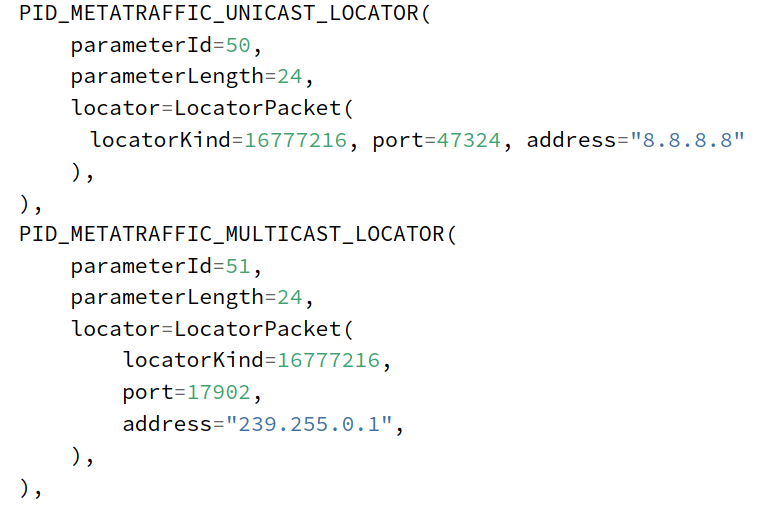
\includegraphics[width=15.2cm, keepaspectratio]{img/submessaggereflection.png}
    \caption{Parte di un pacchetto RTPS costruito con Scapy
    che abilitá un attacco
    riflesso.}
    \label{submessaggereflection}
\end{figure}

Il vettore di questo attacco si trova all'interno di píu parametri 
di un sottomessaggio di tipo DATA. 
Incluso il parametro 
PID\_METATRAFFIC\_MULTICAST\_LOCATOR che si occupa di specificare 
indirizzi multicast che verranno adoperati successivamente dalle 
entità per comunicazioni di metatraffico.
Il DDS non prevede filtri per questo 
specifico valore e quindi un attaccante puó specificare a un 
partecipante di utilizzare un indirizzo IP multicast per il metatraffico 
sotto il suo controllo. Ricevuto questo traffico l'attaccante puó 
ricevere informazioni riguardo la rete DDS e rispondere al partecipante
con un alto numero di comunicazioni in modo tale da sovraccaricarlo (DDoS).

Inoltre, il valore 
di PID\_METATRAFFIC\_MULTICAST\_LOCATOR puó essere anche utilizzato 
da un attore malevolo per reindirizzare il traffico di molteplici 
entitá verso un unico partecipante che si ritoverá quindi a ricevere un 
numero elevato di pacchetti indesiderati rallentandone la sua esecuzione.

Un altro parametro simile é il PID\_METATRAFFIC\_UNICAST\_LOCATOR
che si occupa di specificare un indirizzo Ip di tipo unicast 
per la comunicazioni di metatraffico. Anche in questo caso non é
possibile applicare filtri per limitare la scelta di valori per 
gli indirizzi ip. 

Come mostrato nella 
Figura~\ref{submessaggereflection} creando un pacchetto con Scapy
modificando i valori dei parametri vulnerabili 
é possibile 
rispedire le comunicazioni di una identità verso un qualsiasi
indirizzo, come l'IP del DNS 8.8.8.8 (Figura~\ref{reflectionattackdns}).


\begin{figure}[H]
    \centering
    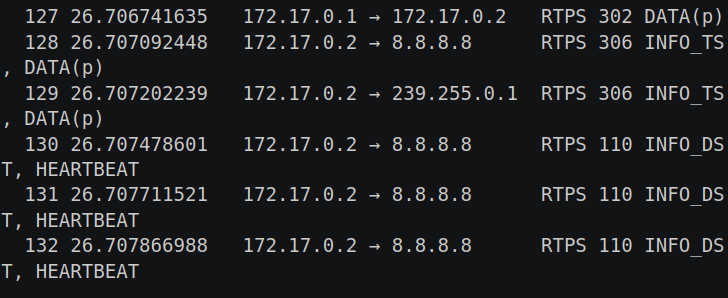
\includegraphics[width=15.2cm, keepaspectratio]{img/reflectionattackdns.png}
    \caption{Esempio di reindirizzamento dei messaggi verso il server DNS 8.8.8.8.}
    \label{reflectionattackdns}
\end{figure}

Questo problema di sicurezza é presente in tutte le implementazioni 
dei vendor dato che non puó essere risolto senza violare lo 
standard OMG. Questa opzione peró, non é considerata dai vari 
vendors perché interromperebbe l'interoperabilità tra le 
diverse implementazioni.
Per rimanere compatibili con lo standard OMG i vendor hanno 
implementato un sistema di controllo che limita il numero 
di pacchetti scambiati quando viene superata una soglia limite
prefissata. Questo sistema non é perfetto, ma in molti casi ha 
ridotto significativamente l'efficacia di questo attacco.

\begin{figure}[H]
    \centering
    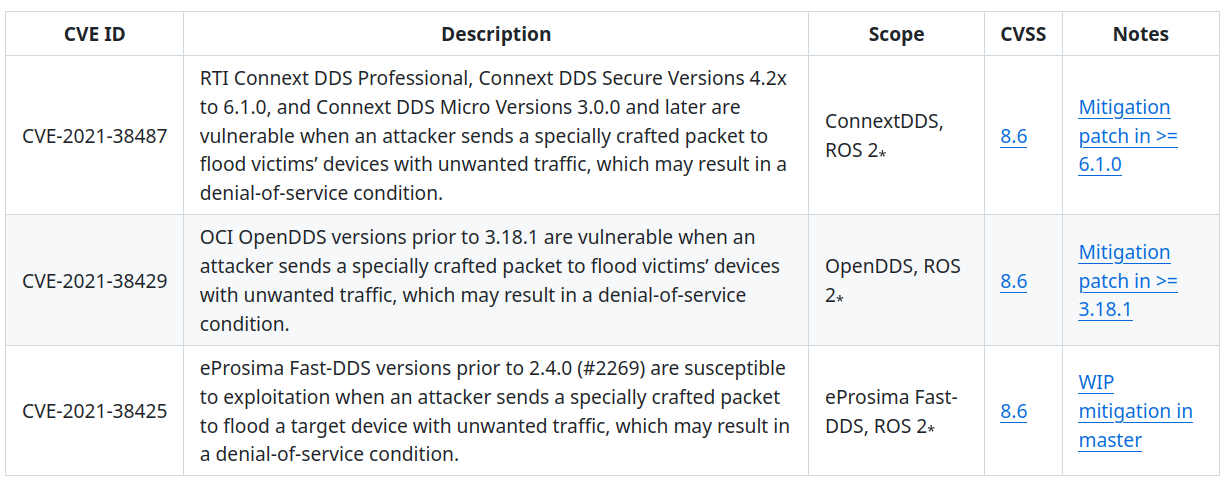
\includegraphics[width=15.2cm, keepaspectratio]{img/CVErecoinnassance.png}
    \caption{Varie CVE per attacco riflesso}
    \label{CVErecoinnassance}
\end{figure}
